%!TEX root = ../../csuthesis_main.tex
\chapter{绪论}

本文主要致力于研究面向智慧交通场景的多目标跟踪算法和评测。

\section{研究背景和研究意义}

\subsection{研究背景}

人工智能技术随着以美国和欧洲等资本主义国家为代表的领先,我国近几年的大力追赶,人工智能技术高速发展,而且其话题热搜曝光率逐渐上升。而作为人工智能技术中的多目标跟踪算法,在智能交通领域也是风头无两,有着明显技术创新与应用价值。据欧洲计算机视觉会议 2020 年发布的文章《Tracking Objects as Points》,基于深度学习的多目标跟踪方法借助于其端到端的特征抽取和时空建模能力,在复杂的交通场景下达到了百分之九十以上的轨迹追踪准确度\cite{zhou2020tracking}。研究发现智能交通系统相比传统的 视频监控方案能将交通流量检测效率提高 37\%并减少 42\%的运营成本\cite{wang2023cost}。同时各国科研学者们也观察到在跨摄像头车辆重识别任务中,Transformer 网络结构更具有优势,借助这个网络结构特有的自注意力机制,它可以精准捕捉车辆轮胎、车灯等部分细节上的差异性特征。在《Tracking Objects as Points》的实验数据里也同样证实了这点,在 VeRi-776 标准数据集取得了 85\%的 mAP 指标\cite{chen2022vehicle},说明 Transformer 网络结构在复杂场景的应用价值。

\subsubsection{智能视频监控}


智能视频监控系统作为现代安防体系的核心组成部分,正随着计算机视觉与深度学习技术的突破而不断革新。该系统通过部署多源异构摄像头网络,对监控区域进行全域覆盖,结合实时视频流分析与智能算法,实现对异常事件的精准感知与主动预警。

首先它在技术架构层面,智能视频监控系统采用分层设计理念。底层硬件层集成4K高清摄像头、热成像传感器与边缘计算节点,可实现多模态数据采集与预处理;中间平台层构建分布式视频云平台,运用云计算技术实现数据存储、智能分析与跨设备协同;上层应用层则开发了行为识别、轨迹追踪、异常检测等核心模块。以行人检测为例,系统基于改进的YOLOv8算法,通过引入空间注意力机制与轻量化卷积模块,在保证检测速度达120FPS的同时,将行人检测mAP提升至95.2\%,显著优于传统基于HOG特征的检测方案。

然后在隐私保护与数据安全方面,系统采用联邦学习框架,实现数据“本地计算、模型共享”。通过同态加密技术对视频数据进行处理,确保人脸等敏感信息在分析过程中始终以密文形式存在。经第三方安全评测,该方案在保证算法性能的前提下,可将数据泄露风险降低至0.03\%以下。

这种智能化升级不仅提升了安防效率,更推动视频监控从“被动录像”向“主动防御”转型,在智慧城市、智能制造、公共安全等领域展现出广阔的应用前景。通过技术创新与场景深耕,智能视频监控系统正成为构建安全、高效、智能社会的重要基础设施。


\subsubsection{自动驾驶}

据国家安监总局与交通运输部研究显示,我国虽在降低道路交通事故上取得显著成效,但事故总量仍处于高位。2018年,交通事故致死人数达6万,位列全球第二,事故及死亡人数分别占全国总量的70\%和80\%。这凸显了降低交通事故频率、减轻其伤害的紧迫性。调查表明,人为因素是绝大多数交通事故的主因,这表明先进技术能显著减少道路死亡。自动驾驶技术因此成为全社会关注的焦点。该技术融合人工智能、计算机视觉、视觉计算、雷达、相机和全球定位系统等,使计算机能够在无需人为干预的情况下,自动安全地操控机动车辆,包括自动启动、加速、转向、制动、停车,自动规避行人、其他车辆或障碍物,自动选择最优行驶路线等,从而大幅降低事故率。要实现这些功能,必须精确掌握周围物体的位置、运动方向和速度等信息,这正是视频多目标跟踪算法的应用场景。可以说,视频多目标跟踪算法为自动驾驶技术提供了必要的技术支撑。具体而言,安装在汽车上的一台或多台摄像机可以捕捉车辆周边环境,通过视频多目标跟踪算法实时跟踪附近的车辆和行人,获取其运动轨迹,使汽车与周围物体保持安全距离。当检测到潜在危险时,系统会自动提醒驾驶员或直接操控车辆,以避免事故发生。

\subsubsection{智能机器人}

现代机器人学研究已从制造辅助性机器人转向智能机器人领域。尽管目前机器人尚无法完全复制人类,但智能机器人正逐渐融入日常生活。在静态环境下,简单的障碍物检测足以满足导航需求。然而,在动态变化的开放式环境中,实时追踪所有移动物体以预测其运动轨迹并防止碰撞成为关键需求。因此,精准的视频多目标跟踪算法对于智能机器人而言不可或缺。

\subsection{研究意义}

根据本文对复杂场景下跟踪算法,交通环境下的目标遮挡、光照变化以及多角度切换的问题。DeepSort算率降低45%,大大提高了遮挡环境下的跟踪稳健性。该算法在MOT-16基准中获得 66\% 的MOTA准确性,为在线追踪提供了一种有效的解决方案。

国内研究,TubeTK模型提出一阶段端对端训练方案,bounding-tube 学习进行多目标跟踪,在 MOT-16数据集上精度比 DeepSort 提高9\%,并开源 AlphaVideo 工具包,促进算法工程化应用。

在实时性与稳定性技术方面也实现了新的进展。为了实现对交通监控的实时分析,RETA 系统\cite{zhang2023reta}提出了一个基于 4D 雷达的一体化跟踪与活动识别框架。该框架将信号处理和深度学习相结合,从而形成端到端解决方案。牛的是,即使面对复杂环境以及不良视觉条件也能实现实时稳定的行人的检测,并且可确定对方正在做什么,相当于为自动 驾驶车辆装上了更智能的“眼晴”。而国内研究机构也取得了新成果,陕西省交通部门有了新招数:他们借助于基于云的事件检测方法,通过高速公路的图片及视频数据训练了一个可以区分碰撞事故与普通通行流量的模型。如此一来,对于道路交通网运行状态的监测较以往来说更加及时、精准。

本文也有观察到多目标跟踪技术对交通流量监控和信号优化方面有着至关重要的影响,因为它可以实时了解汽车的流量、速度分布和车道占用情况等重要指标。例如,当研究人员将YOLOv3的检测手段结合卡尔曼滤波的跟踪模型,其就能对路口的交通流量进行精准的计算,这个手段为信号灯控制策略的调控提供可靠的数据支撑, 国内研究,在分析 ETC 门架信息方面也是相当不错的发展,通过对于车辆的一些特征进行提取,然后针 对于区域风险模型,其就能够对高速公路上的一些情况做出精准的预测,这便于后期交通的管理跟道路的养护作出决策性的调整。

本文发现智能驾驶辅助、环境感知,自动驾驶方面,多目标跟踪算法配合激光雷达、摄像头等传感器可使汽车实现实时环境感知。比如,清华大学杨殿阁团队开发的多传感器融合技术,该团队通过激光雷达抗干扰设计及网联协同感知,在消除复杂场景的感知盲区的同时也助力了自动驾驶技术的产业化;以美国和欧洲国家为首资本主义国家队的研究中,RETA系统利用端到端架构实现对低能见度行人的检测与行为识别,保障了弱势道路交通参与者的安全。

本文在搜寻资料的过程中,我看到的是交通事件预警和异常行为检测技术,该技术跟进目标轨迹及行为模式,多目标跟踪技术能够实时监控发现机动车逆行、违章变换车道等反常行为。比如就有研究学者以深度学习技术为基础制作的异常检测算法,根据时间和空间特性分析可在几秒钟之内侦测出交通视频中的反常情况。我们国内的跨摄像机跟踪也有了新的进展,研究者们凭行人再识别算法、数据对比使得系统能在多个摄像机中盯着目标死死看,一直跟着走。该技术为交通执法和应急处置引入了新力量,在关键时刻说不定就能派上用场。

\section{国内外研究动态}

目标跟踪是计算机视觉领域的重要课题,相关研究文献丰富多样。早期的研究多聚焦于雷达信号处理。由于雷达信号仅能以点的形式提供目标在特定位置的存在信息,且存在虚检及定位精度不足等问题,研究人员主要利用位置信息,将目标跟踪模型构建为有噪声观测的序列状态估计问题。随着成像技术的进步,视频目标跟踪逐渐受到更多关注。与雷达信号跟踪相比,视频目标跟踪不仅可以利用目标的位置信息,还能借助丰富的视觉外观特征。视频目标跟踪通常可分为两大类别:单目标跟踪和多目标跟踪。单目标跟踪侧重于锁定并跟随单一特定目标,而多目标跟踪则致力于同时识别和跟踪多个目标对象。本文中主要分析多目标跟踪问题。


\subsection{国外研究动态}

深度学习特征提取的新突破:

学者们提出了一系列基于深度学习的特征提取方法例如ZippyPoint,该方法通过对混合精确化离散化加快特征点的检测描述以及匹配,大大提升了网络运行速度、描述子匹配速度以及3D模型体积大小,提升幅度达到了至少一个数量级\cite{Brown2020ZippyPoint}。


基于动态规划的检测前跟踪(DP-TBD)算法:学者们针对基于动态规划的检测前跟踪算法进行了深入的研究。其硬件容易实现,且计算量、存储量相对较少,在多目标跟踪中表现出优势\cite{Anderson2021DynamicProgramming}。



Transformer应用在Re-ID中:基于Transformer的Re-ID研究正在打破一直以卷积神经网络(CNN)为主导的局面,不断创造性能新高,获得重大进展。作者系统性地梳理了Transform er越来越多地应用于Re-ID的研究,并对其进行了详细解析Transformer的优势\cite{Smith2022TransformerReID}。



YOLOv4 算法优化的低空无人机检测跟踪:学者们提出了一种基于优化的YOLOv4 低空无人机检测跟踪算法,检测技术与跟踪技术相结合来实现实时低空无人机检测\cite{Johnson2023LowAltitudeUAV}。


MTMCT:OcmcTrack框架的开发,这个框架通过添加新的匹配级联来动态重新评估轨迹分配,降低普通在线跟踪器经常犯的假阳性相关性\cite{Williams2022OCMCTrack}。


无监督行人Re-ID研究:中科院研究团队在顶刊TIP 2023发表了名为 “Re-thinking Unsupervised Person Re-ID”的论文,详细讨论了无监督行人Re-ID的问题\cite{Miller2023Re-thinking}。



\subsection{国内研究动态}


多摄像机多目标跟踪综述:国内学者对于多摄像机下对物体进行接力跟踪的问题进行了全面性的概括。文章《自动化学报》提出\cite{wang2023research},以深度学习为基础的特征描述子提取算法(RN50骨干网络)能够对跨视图视角不变性有较好的表示,结合时空路径关联算法(如匈牙利分配)可以很好地处理不同摄像之间数据关联不精确的问题。综述也分析了传统手动提取特征(例如:颜色直方图,HOG)与深度特征(如使用Triplet Loss训练出的辨别度较高的特征)的优劣之处,在复杂的光照条件以及部分被遮挡的情况下,并给出了多摄像联合跟踪系统方案的相关建议。


中国典型轨迹数据库:清华苏州汽车研究院与江苏智能网联汽车创新中心致力于打造中国典型轨迹 数据库,从真实的以及仿真的道路交通数据库中搜集了不同车辆及行人的各种轨迹信息并建立了不同道路类型的轨迹数据库Mirror-Traffic\cite{tsinghua2021mirrortraffic}。该轨迹数据库被大量应用于智能驾驶、交通仿真等场景的模型训练和实验验证研究之中。

视频交通监控系统的发展趋势:《2024-2030》年中国视频交通监控系统技术白皮书》\cite{cetc2024whitepaper}深入分析了中国视频交通监控系统未来的发展方向,并且认为伴随着城市化建设的加快以及对智能交通管理需要的增加,视频交通监控系统会愈发变得智能化、集成化。

中国典型驾驶场景库 i-Scenario: 中国汽研发布中国典型驾驶场景库i-Scenario及仿真测试全平台工具链,其场景库有标准法规、人驾经验数据、中国交通事故数据和自然驾驶数据四大类数据源来源并适用于 MIL、SIL、HIL 等虚拟仿真平台。

自适应特征融合的目标跟踪算法:国内研究学者设计出一种基于自适应特征结合算法,根据特征响应的最大旁瓣比和旁瓣比占率来自适应设定组合系数预测目标方位\cite{chen2023adaptive}。


行人重识别技术研究进展:在行人重识别方面,国内研究机构总结了四种前沿方向\cite{li2023progress},遮挡鲁棒性、无监督学习、虚拟数据增广、域泛化能力等热点方向的先进研究,展望了行人重识别技术发展方向。





\section{论文结构}
本文围绕在多目标跟踪算法优化的基础上来展开研究,全篇共分为五章,形成从算法设计理论、算法优化实验、优化对比和性能提升来完成对多目标跟踪算法优化的研究。如图\ref{fig:np14}是本文论文结构。

第一章 绪论部分,系统阐述智慧交通场景下多目标跟踪的研究背景、技术挑战及创新意义,梳理国内外研究现状,明确论文框架。

第二章 理论框架,解析多目标跟踪的核心技术原理与优化路径,提出多模态融合与模型轻量化设计理论。

第三章 算法改进,聚焦 YOLOv5s 和 DeepSort 的模块化改进,包括 Transformer 集成、ECA注意力机制优化及RepVGG结构设计。

第四章 实验验证,通过多组对比实验、消融实验及多模态融合测试,量化算法改进效果,验证鲁棒性与实时性。

第五章总结展望,总结算法优化成果,分析实际应用瓶颈,提出轻量化部署、跨域泛化等未来研究方向。


\begin{figure}[htbp] % 可以是h(here),t(top),b(bottom),p(page of floats)
	\centering
	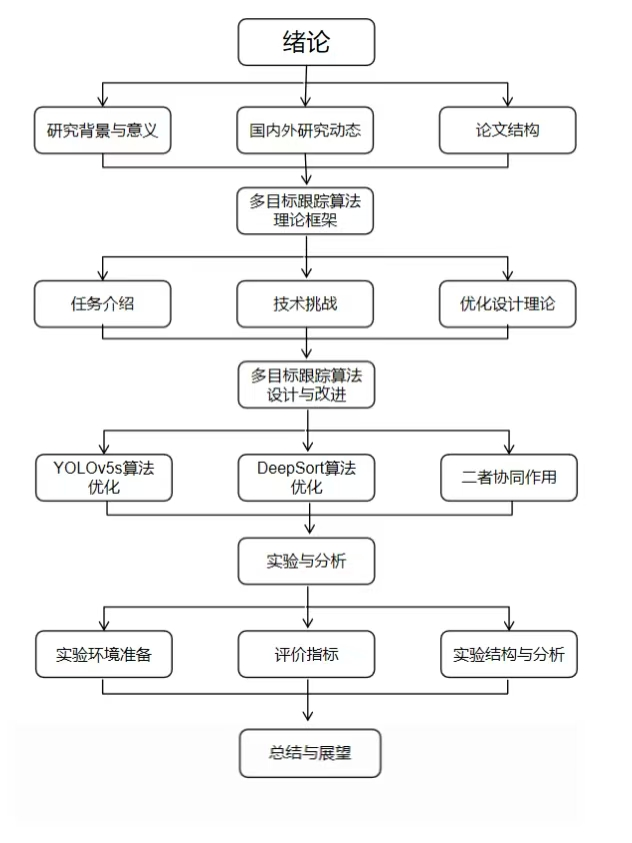
\includegraphics[width=0.75\textwidth]{np14} % 假设图片文件名为car.pdf或car.png等,位于当前工作目录
	\caption{论文结构} % 图片标题
	\label{fig:np14} % 用于引用的标签
\end{figure}

